\documentclass[class=book, crop=false, oneside, 12pt]{standalone}
\usepackage{standalone}
\usepackage{../../style}
\graphicspath{{./assets/images/}}

% arara: pdflatex: { synctex: yes, shell: yes }
% arara: latexmk: { clean: partial }
\begin{document}
\chapter{Proprietà dei linguaggi liberi}
È il momento di fare una gita domenicale di famiglia presso il supermercato MondoMatematica\textregistered e perderci tra i gli scaffali invitanti e variopinti, stregati dalla capitalistica attrazione che tutte quelle proprietà, quei lemmi e quei teoremi esercitano su di noi.
  
\section{Proprietà di chiusura}
\subsection*{Chiusura rispetto all'unione}
\begin{lemma}
  La classe dei linguaggi liberi è chiusa rispetto all'operazione di unione d'insiemi.
  \begin{equation*}
    \textrm{Se } \mathcal{L}_1 \textrm{ è libero} \land \mathcal{L}_2 \textrm{ è libero} \implies \mathcal{L}_1 \cup \mathcal{L}_2 \textrm{ è libero}
  \end{equation*}
\end{lemma}

\begin{proof}
    Siano \(\mathcal{L}_1\) e \(\mathcal{L}_2\) dei linguaggi liberi; questo vuol dire che devono esistere due grammatiche libere, ciascuna delle quali ha generato uno dei due linguaggi. In simboli:

  \begin{equation*}
    \exists\; \mathcal{G}_1 = (V_1, T_1, S_1, \mathcal{P}_1), \mathcal{G}_2 = (V_2, T_2, S_2, \mathcal{P}_2) : \mathcal{L}_1 = \mathcal{L}(\mathcal{G}_1) \textrm{ e } \mathcal{L}_2 = \mathcal{L}(\mathcal{G}_2)
  \end{equation*}

  Vediamo quindi come costruire una nuova grammatica libera che possa generare l'unione dei due linguaggi generati dalle rispettive grammatiche viste sopra. Consideriamo quindi una nuova grammatica \(\mathcal{G}\), i cui elementi sono così definiti:

  \begin{equation*}
      \mathcal{G} = (V'_1 \cup V'_2 \cup \{S\}, T_1 \cup T_2, S, \mathcal{P}'_1 \cup \mathcal{P}'_2 \cup \{S \rightarrow S'_1 \mid S'_2\})
  \end{equation*}

  \noindent Andiamo a vedere da vicino come sono stati ricavati gli elementi:

  \begin{itemize}
    \item \(V'_1\) e \(V'_2\) si ottengo effettuando un'operazione di \emph{refresh} sui non terminali, in modo da evitare collisioni di nomi (vedremo più avanti come mai quest'operazione è importante), inoltre questo vocabolario è completato con l'introduzione di un nuovo start symbol;
    \item l'insieme dei terminali è l'unione dei sue insiemi di terminali di \(\mathcal{G}_1\) e \(\mathcal{G}_2\);
    \item \(S\) è il nuovo start symbol, non presente in \(V'_1 \cup V'_2\), e \(S'_1\) e \(S'_2\) sono di nuovo il refresh degli start symbol rispettivamente di \(\mathcal{G}_2\) e \(\mathcal{G}_2\);
    \item infine, l'insieme delle produzioni è dato dall'unione tra i refresh delle produzioni delle due grammatiche di partenza  \(\mathcal{G}_1\) e \(\mathcal{G}_2\), unito a una nuova produzione che, dal nuovo start symbol, produce il resfresh dello start symbol di una delle due grammatiche di partenza.
  \end{itemize}

  \noindent Questa definizione ci basta per asserire che \(\mathcal{L(G)}\) è libero e \(\mathcal{L(G)} = \mathcal{L}(\mathcal{G}_1)  \cup \mathcal{L}(\mathcal{G}_2) \).

\end{proof}

\begin{osservazione}
  Cerchiamo di capire come mai possiamo essere certi che la grammatica \(\mathcal{G}\), per come l'abbiamo definita, è libera.

  Prendiamo l'insieme delle produzioni di \(\mathcal{G}\); abbiamo già visto come è stato ricavato. Il refreshing va a colpire solamente i nomi dei terminali o non-terminali, non la forma delle produzioni che li interessano, la quale rimane immutata (\(A \rightarrow \alpha\)). Questa forma è rispettata anche dalle due nuove produzioni aggiunte (\(S \rightarrow S'_1\) e \(S \rightarrow S'_2\)) e quindi non vengono introdotte produzioni che rendono la grammatica context dependent.

\end{osservazione}

\begin{osservazione}
  Cerchiamo di capire come mai  \(\mathcal{L(G)} = \mathcal{L}(\mathcal{G}_1)  \cup \mathcal{L}(\mathcal{G}_2) \) è valido.
  \begin{itemize}
    \item Consideriamo una stringa \(w \in \mathcal{L(G)}\); questo è vero se e solo se esiste una certa derivazione per ottenerla a partire dallo start symbol (\(S \implies^* w\)).
    \item Per come abbiamo definito la grammatica \(\mathcal{G}\), il secondo passo della derivazione dev'essere necessariamente il refresh di uno dei due start symbol delle grammatiche di partenza (\(S \implies S'_1 \implies^* w \lor S \implies S'_2 \implies^* w\));
    \item questo naturalmente è valido se e solo se, a questo punto, la stringa \(w\) può essere derivata in qualche modo a partire da uno degli start symbol delle grammatiche di partenza (\(S_1 \implies^* w \lor S_2 \implies^* w\)).
    \item Se \(w\) può essere ottenuta attraverso qualche derivazione a partire da \(S_1\) o \(S_2\), allora vuol dire che \(w\) appartiene a uno dei due linguaggi generati dalle nostre due grammatiche di partenza (\(w \in \mathcal{L}(\mathcal{G}_1)  \lor w \in \mathcal{L}(\mathcal{G}_2) \)).
    \item Questo è equivalente ad affermare che \(w\) appartiene all'unione dei due linguaggi (\(w \in \mathcal{L}(\mathcal{G}_1)  \cup \mathcal{L}(\mathcal{G}_2) \)), e ci convince quindi della validità dell'asserto.
  \end{itemize}
\end{osservazione}

\begin{osservazione}
  È semplice convincersi dell'importanza dell'operazione di refreshing. Se consideriamo due grammatiche \(\mathcal{G}_1, \mathcal{G}_2\) con le seguenti produzioni:
  % \begin{figure}
  %   \centering
  %   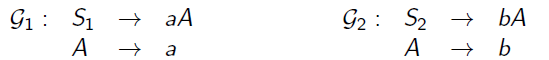
\includegraphics[width=.7\textwidth,keepaspectratio]{why-refresh_1}
  % \end{figure}

  \begin{align*}
    \mathcal{G}_1: S_1\; &\to\; aA & \mathcal{G}_2: S_2\; &\to\; bA \\
    A\; &\to\; a & A\; &\to\; b
  \end{align*}

  \noindent Avremo quindi generati i seguenti linguaggi: \(\mathcal{L}(\mathcal{G}_1)  = \{aa\}\) e \(\mathcal{L}(\mathcal{G}_2)  = \{bb\}\).

  Se non effettuassimo refreshing, ci troveremo ad avere una nuova grammatica con le seguenti produzioni:
  % \begin{figure}
  %   \centering
  %   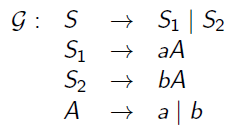
\includegraphics[width=.3\textwidth,keepaspectratio]{why-refresh_2}
  % \end{figure}

  \begin{align*}
    \mathcal{G}: S\; &\to\; S_1\; \mid S_2 \\
    S_1\; &\to\; aA \\
    S_2\; &\to\; bA \\
    A\; &\to\; a\; \mid b
  \end{align*}

  \noindent Il linguaggio prodotto da questa nuova grammatica sarebbe diverso da quello dato dall'unione delle due grammatiche di partenza, poiché avremmo \(\mathcal{L(G)} = \{aa, ab, ba, bb\} \neq \mathcal{L}(\mathcal{G}_1)  \cup \mathcal{L}(\mathcal{G}_2) \).

  Con un'opportuno resfreshing otteniamo invece:
  % \begin{figure}
  %   \centering
  %   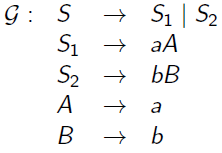
\includegraphics[width=.3\textwidth,keepaspectratio]{why-refresh_3}
  % \end{figure}

  \begin{align*}
    \mathcal{G}: S\; &\to\; S_1\; \mid S_2 \\
    S_1\; &\to\; aA \\
    S_2\; &\to\; bB \\
    A\; &\to\; a \\
    B\; &\to\; b
  \end{align*}

  Questo insieme di produzioni garantisce che la grammatica generi il linguaggio desiderato.
\end{osservazione}

\subsection*{Chiusura rispetto alla concatenazione}

\begin{lemma}
  La classe dei linguaggi liberi è chiusa rispetto all'operazione di concatenazione.

  \begin{equation*}
    \textrm{Se } \mathcal{L}_1 \textrm{ è libero} \land \mathcal{L}_2 \textrm{ è libero} \implies \{w_1w_2 \mid w_1 \in \mathcal{L}_1 \land w_2 \in \mathcal{L}_2\} \textrm{ è un linguaggio libero.}
  \end{equation*}

\end{lemma}

\begin{proof}% La dimostrazione sembra assolutamente uguale a quella del lemma della chiusura all'unione, sono confuso ma domani cercherò di chiarire.Alla fine ha chiarito il Sam, grazie Sam.\\
  Consideriamo due linguaggi liberi \(\mathcal{L}_1\) e \(\mathcal{L}_2\); ciò implica che esistano due grammatiche libere \(\mathcal{G}_1\) e \(\mathcal{G}_2\) che soddisfano la seguente equazione:
  \begin{equation*}
    \exists\; \mathcal{G}_1 = (V_1, T_1, S_1, \mathcal{P}_1), \mathcal{G}_2 = (V_2, T_2, S_2, \mathcal{P}_2) : \mathcal{L}_1 = \mathcal{L}(\mathcal{G}_1) \textrm{ e } \mathcal{L}_2 = \mathcal{L}(\mathcal{G}_2)
  \end{equation*}
  Consideriamo quindi una nuova grammatica \(\mathcal{G}\), i cui elementi sono così definiti:

  \begin{equation*}
      \mathcal{G} = (V'_1 \cup V'_2 \cup \{S\}, T_1 \cup T_2, S, \mathcal{P}'_1 \cup \mathcal{P}'_2 \cup \{S \rightarrow S'_1 S'_2\})
  \end{equation*}
  La definizione dei vari elementi della precedente equazione procede pari passo a quella già vista nel lemma della chiusura rispetto all'unione.
  L'unica differenza è la definizione del linguaggio \(\mathcal{L}(\mathcal{G})\) che appunto qui è costruito per concatenazione e non per unione:
  \begin{equation*}
    \mathcal{L(G)} = \{w_1 w_2 \mid w_1 \in \mathcal{L}(\mathcal{G}_1) \land w_2 \in \mathcal{L}(\mathcal{G}_2) \}
  \end{equation*}
  La dimostrazione del lemma di chiusura rispetto alla concatenazione procede pari passo a quella del lemma di chiusura rispetto all'unione, di conseguenza non è qui riportata. 
\end{proof}

\subsection*{Chiusura rispetto all'interezione}

\begin{lemma}
  La classe dei linguaggi liberi non è chiusa rispetto all'operazione d'intersezione.
\end{lemma}

\begin{proof}
  La dimostrazione è per contraddizione, è sufficiente trovare due linguaggi liberi la cui intersezione non è libera.

  Si considerino, ad esempio, due linguaggi \(\mathcal{L}_1\) e \(\mathcal{L}_2\), definiti come segue:
  \begin{align*}
      \mathcal{L}_1 = \{a^n b^n c^j \mid n, j > 0 \} \\
      \mathcal{L}_2 = \{a^j b^n c^n \mid n, j > 0 \}
  \end{align*}

  \noindent Il linguaggio generato dalla loro intersezione è il seguente:

  \begin{align*}
    \mathcal{L}_1 \cap \mathcal{L}_2 = \{ a^n b^n c^n \mid n > 0 \}
  \end{align*}

  \noindent Questo linguaggio non è libero, e provarlo è molto semplice (si veda Tab.~\ref{tab:ex-freeNotFree_1}).

\end{proof}

\section{Chomsky Normal Form}
\paragraph{Definizione}
Una grammatica libera \(\mathcal{G} = (V, T, S, \mathcal{P})\) è in \emph{Chomsky Normal Form} se e solo se:
\begin{itemize}
  \item non ha alcuna \(\varepsilon\)-produzione, al massimo \(S \rightarrow \varepsilon\);
  \item tutte le sue non \(\varepsilon\)-produzioni hanno una tra le due seguenti forme:
  \begin{itemize}
    \item \(A \rightarrow a\)
    \item \(A \rightarrow BC\)
  \end{itemize}
  in cui sia \(B\) sia \(C\) sono diversi da \(S\).
\end{itemize}

\begin{lemma}
  Sia \(\mathcal{G}\) una grammatica libera; allora esiste una certa grammatica \(\mathcal{G'}\) in Chomsky Normal Form tale che \(\mathcal{L(G)} = \mathcal{L(G')}\).
\end{lemma}

\noindent La dimostrazione del lemma è lasciata per esercizio.

\section{Come epurare le grammatiche libere}
Esiste un teorema che ci permette di fare pulizia etnica sui linguaggi.
\begin{theorem}
  Consideriamo un linguaggio libero \(\mathcal{L}\); allora esiste una grammatica libera \(\mathcal{G}\) tale che \(\mathcal{L(G)} = \mathcal{L} \setminus \{ \varepsilon \}\) e tale da:
  \begin{itemize}
    \item non avere alcuna \(\varepsilon\)-produzione, ovvero produzioni di forma \(A \rightarrow \varepsilon\);
    \item non avere alcuna produzione d'unità (\emph{unit production}), ovvero produzione di forma \(A \rightarrow B\);
    \item non avere alcun non-terminale non utile, ovvero non-terminali che non appaiono mai in alcuna derivazione di qualche stringa di terminale.
  \end{itemize}
\end{theorem}

Le grammatiche che possiedono queste caratteristiche sono più sintetiche e generano linguaggi equivalenti a livello espressivo, ma più puliti; ad esempio, non c'è alcun bisogno di avere non-terminali che abbiano una produzione in \(\varepsilon\) e, qualora richiesto, la produzione \(S \rightarrow \varepsilon\) sarebbe sufficiente allo scopo, spiegheremo in seguitoquesta affermazione.

Non è nostro interesse entrare nel dettaglio degli algoritmi per effettuare questa pulizia, poiché dimostrarne la correttezza richiederebbe un considerevole impegno. Andremo però ad analizzare come possiamo, se non altro,  eliminare le \(\varepsilon\)-produzioni.

\subsection{Come eliminare le produzioni di parole vuote}
Per eliminare le \(\varepsilon\)-produzioni bisogna procedere ad individuare i non-terminali \emph{annullabili} (\emph{nullable}), ovvero quei non-terminali che, con qualche derivazione, producono la parola vuota (\(A : A \rightarrow^\ast \varepsilon\)). Si può procedere ricorsivamente:
\begin{description}
  \item[Base] se la grammatica comprende una produzione della forma \(A \rightarrow \varepsilon\), allora quel non-terminale \(A\) è annullabile;
  \item[Step] se la grammatica comprende una produzione della forma \(A \rightarrow Y_1Y_2 \ldots Y_n\) e i non terminali \(Y_1, Y_2, \ldots, Y_3\) sono tutti annullabili, allora anche \(A\) è annullabile. 
\end{description}
A questo punto, andiamo a sostituire ogni produzione della forma \(A \rightarrow Y_1Y_2 \ldots Y_n\) con una famiglia di produzioni dove ogni combinazione di \(Y_i\) annullabili è rimossa dal body della produzione. Se tutti gli \(Y_i\) sono annullabili, la stessa produzione \(A \rightarrow Y_1Y_2 \ldots Y_n\) diventa di questa forma \(A \rightarrow \varepsilon\) e non viene quindi inclusa nelle produzioni finali. Quindi, si elimina ogni produzione \(A \rightarrow \varepsilon\).

\paragraph{Esempio di applicazione}
Andiamo a vedere un esempio considerando la seguente grammatica:
%
% \begin{figure}
%   \centering
%   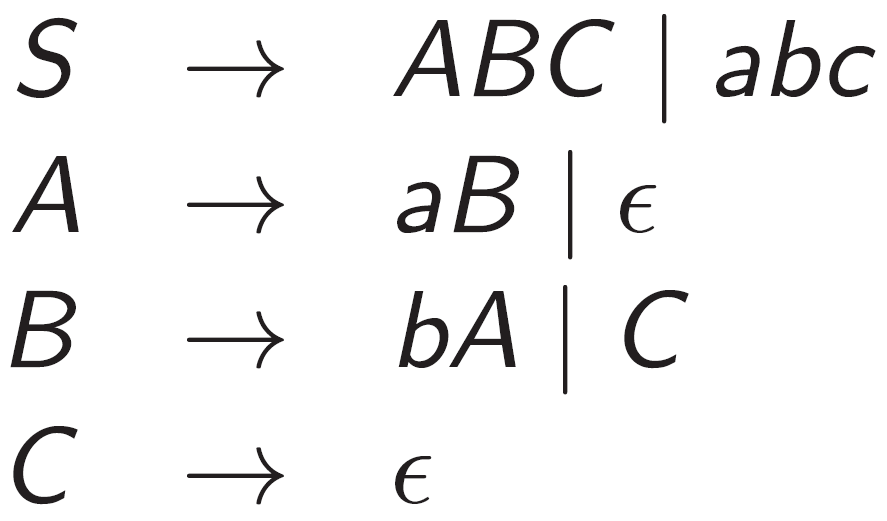
\includegraphics[width=.3\textwidth,keepaspectratio]{ex-th-1-3-1_1}
% \end{figure}

\begin{align*}
  S\; & \to\; ABC\; \mid abc \\
  A\; & \to\; aB\; \mid \varepsilon \\
  B\; & \to\; bA\; \mid C \\
  C\; & \to\; \varepsilon
\end{align*}

Osserviamo subito che \(C\) ha solo una produzione e questa conduce a \(\varepsilon\), pertanto è annullabile; allo stesso modo, \(B\) è annullabile attraverso \(C\) e \(S\) è annullabile attraverso \(A, B\) e \(C\). Con le operazioni che abbiamo illustrato poc'anzi, la grammatica che otteniamo è la seguente:

% \begin{figure}
%   \centering
%   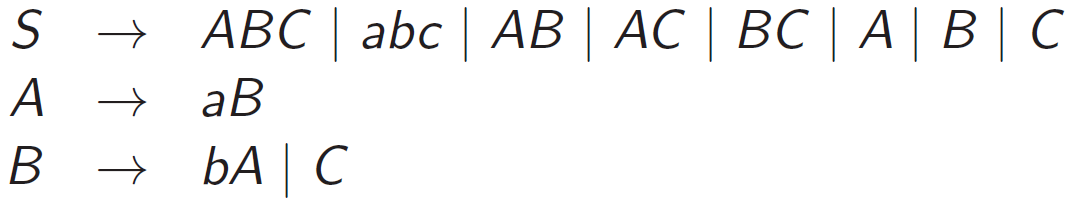
\includegraphics[width=.3\textwidth,keepaspectratio]{ex-th-1-3-1_2}
% \end{figure}

\begin{align*}
  S\; & \to\; ABC\; \mid abc\; \mid AB\; \mid AC\; \mid BC\; \mid A\; \mid B\; \mid C \\
  A\; & \to \; aB \\
  B\; & \to\; bA\; \mid C
\end{align*}

Si noti che, in questa grammatica, il non-letterale \(C\) è non utile.

\section{Pumping lemma per linguaggi liberi}
\subsection{Definizione e formulazione}
Si segua lentamente formulazione e dimostrazione per questo tanto articolato quanto importante lemma.
\begin{lemma}
  Consideriamo un linguaggio libero \(\mathcal{L}\), allora:
  \begin{itemize}
    \item \(\exists p \in \mathbb{N}^+\) tale che
    \item \(\forall z \in \mathcal{L} : |z| > p\), allora
    \item \(\exists u, v, w, x, y\) tale che:
    \begin{itemize}
      \item \(z = uvwxy \textrm{ } \land\)
      \item \(|vwx| \leq p \textrm{ } \land\)
      \item \(|vx| > 0 \textrm{ }\land\)
      \item \(\forall i \in \mathbb{N}.uv^iwx^iy \in \mathcal{L}\)
    \end{itemize}
  \end{itemize}
\end{lemma}
\begin{proof}
  Partiamo considerando un linguaggio libero \(\mathcal{L}\) che non comprende la parola vuota (\(\varepsilon \notin \mathcal{L}\)); sappiamo quindi che deve esistere una grammatica libera "epurata" \(\mathcal{G}\) che generi il linguaggio \(\mathcal{L}\) (\(\mathcal{L} = \mathcal{L(G)}\)).

  Osserviamo che, per ogni possibile albero di derivazione, ogni cammino dalla radice a un terminale attraversa tanti non-terminali quanto il valore della lunghezza del cammino stesso. Ad esempio, la lunghezza del cammino \(\langle S, B_1, B_2, \ldots, B_{k-1}, a \rangle\) è \(k\), così come il numero di non-terminali attraversati.

  Adesso definimo \(p\) come la lunghezza della più lunga parola derivabile con degli alberi di derivazione, e che inoltre sia tale che i suoi camini, a partire dalla radice, siano lunghi al più come il numero di non-terminali di \(\mathcal{G}\). Consideriamo quindi anche una parola \(z \in \mathcal{L}\), più lunga di \(p\) (\(|z| > p\)). Possiamo quindi essere sicuri che esiste un albero di derivazione per \(z\) che possiede almeno un cammino la cui lunghezza è strettamente maggiore del numero di non-terminali, poiché \(|z| >p\).

  Adesso, per un qualche albero di derivazione, andiamo a considerare la più profonda coppia di occorrenze dello stesso non-terminale lungo un qualche cammino; con più profonda coppia di occerrenze intendiamo la coppia composta dalla più lontana e dalla seconda più lontana occorrenza dalla radice di uno stesso non terminale.

  Andiamo a visualizzare la situazione attraverso un albero di derivazione, considerando le due occorrenze di un non-terminale \(A\).
  \begin{figure}
    \centering
    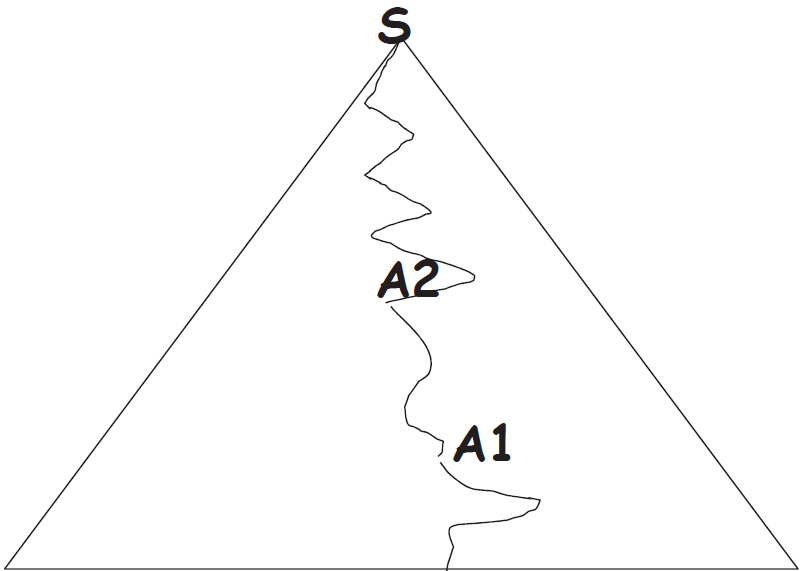
\includegraphics[width=.25\textwidth,keepaspectratio]{pl-proof_1}
  \end{figure}
  Possiamo dire, nelle due occorrenze di \(A\), sono radicati due sottoalberi distinti, che noi qui rappresenteremo colorati di verde e porpora. La parola \(z\) può quindi essere "spacchettata" in cinque sottoparole, come illustrato di seguito.
  \begin{figure}
    \centering
    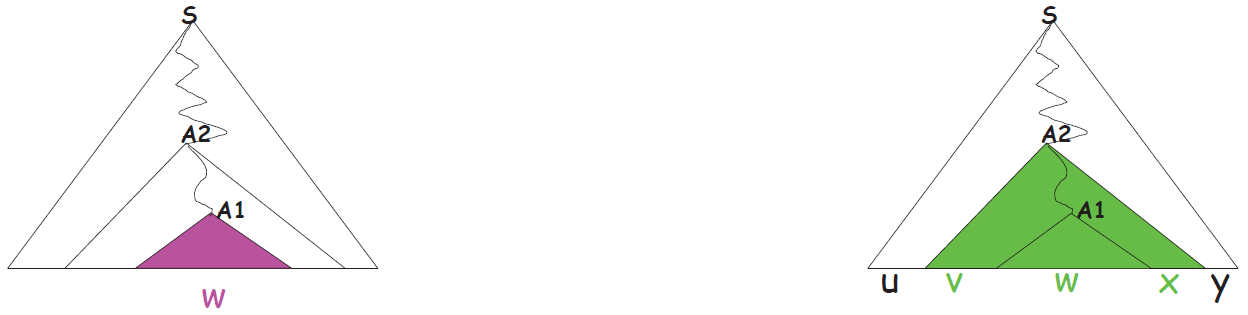
\includegraphics[width=.8\textwidth,keepaspectratio]{pl-proof_2}
  \end{figure}
  Dal momento che \(A_1\) e \(A_2\) sono occorrenze di uno stesso non-terminale, condividono la medesima famiglia di produzioni. Questo fatto è notevole: se, a partire da \(A_2\), siamo riusciti a trovare una qualche sequenza di derivazioni tale da essere arrivati a \(A_1\), allora con la stessa sequenza possiamo trovare una nuova occorrenza di \(A\), il che ci rende ragionevolmente certi che possiamo generare un numero arbitrario di sottostringhe \(v, x\) di \(z\).
  \begin{figure}[H]
    \centering
    \begin{minipage}{0.25\textwidth}
      \centering
      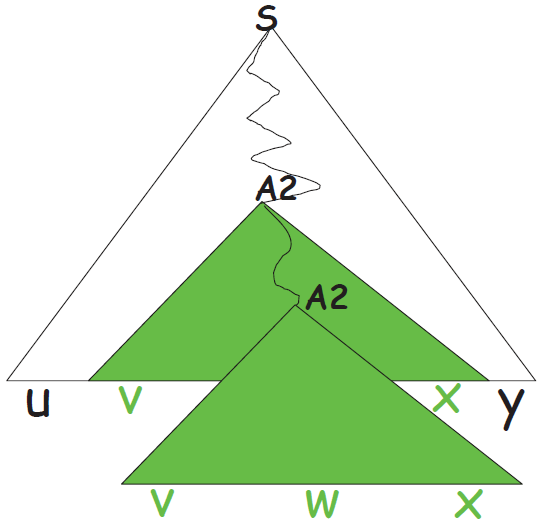
\includegraphics[width=\textwidth,keepaspectratio]{pl-proof_3}
    \end{minipage}
     \hfill
    \begin{minipage}{0.25\textwidth}
      \centering
      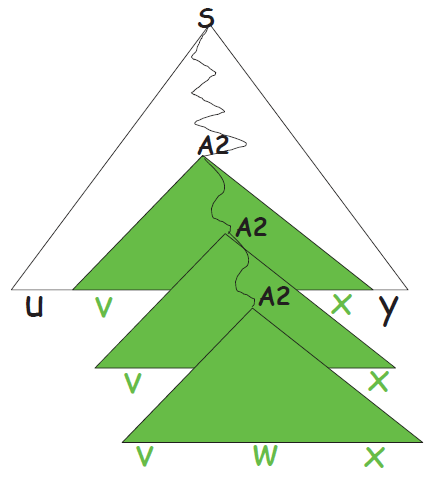
\includegraphics[width=\textwidth,keepaspectratio]{pl-proof_4}
    \end{minipage}
  \end{figure}
  Allo stesso modo sappiamo che, se a partire da \(A_1\) possiamo ottenere un sottoalbero di derivazioni \(w\), questo stesso sottoalbero può essere ottenuto a partire da \(A_2\).
  \begin{figure}
    \centering
    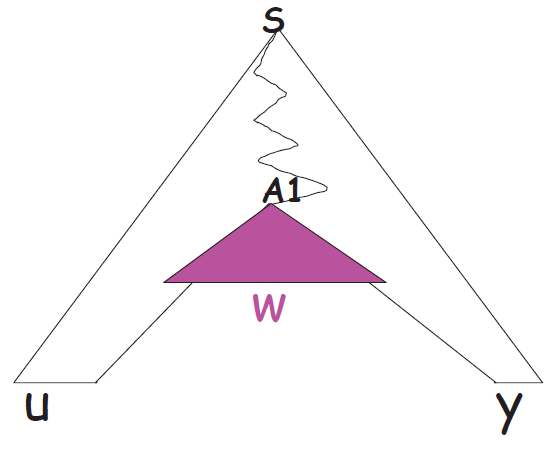
\includegraphics[width=.25\textwidth,keepaspectratio]{pl-proof_5}
  \end{figure}
  Queste affermazioni possono essere riassunte, per l'appunto, nella formula:
  \begin{equation*}
    \forall i \in \mathbb{N}.uv^iwx^iy \in \mathcal{L}
  \end{equation*}
  Ulteriori considerazioni:
   \begin{itemize}
     \item per come abbiamo scelto le occorrenze di \(A\), la profondità del sottoalbero radicato in \(A_2\) è minore del numero di non-terminali presenti nella grammatica considerata, da cui, per definizione stessa del valore \(p\), \(|vwx| < p\);
     \item la grammatica \(\mathcal{G}\) che genera il linguaggio che stiamo considerando è ripulita, per cui nelle derivazioni di forma \(A \implies^* \alpha A \beta\), almeno uno dei due simboli \(\alpha, \beta\) deve fornire uno ulteriore; questo ci permette di affermare che \(|vx| > 0\).
   \end{itemize}

   \paragraph{Dimostrazione se \(\varepsilon \in \mathcal{L}\)}
   La dimostrazione che abbiamo appena concluso è relativa a linguaggi privi di parola vuota, ma con un attimo di cura nell'impostazione possiamo estenderla anche ai linguaggi che comprendono \(\varepsilon\).

   Considerando un linguaggio \(\mathcal{L}\) che comprenda \(\varepsilon\), partiamo ricavando una grammatica \(\mathcal{G} = (V, T, S, \mathcal{P})\) che generi \(\mathcal{L} \setminus \{\varepsilon\}\). A questo punto definiamo una seconda nuova grammatica \(\mathcal{G}'\), in cui andiamo semplicemente ad aggiungere un nuovo start symbol assieme a due produzioni: una che punti verso lo start symbol della precedente grammatica, e una seconda che generi invece \(\varepsilon\). Formalmente:

   \begin{equation*}
     \mathcal{G}' = (V, T, S', \mathcal{P} \cup \{ S' \rightarrow S, S' \rightarrow \varepsilon \})
   \end{equation*}

   In questo modo abbiamo che \(\mathcal{L} = \mathcal{L(G')}\) e possiamo procedere analogamente a prima

\end{proof}

\subsection{Applicazioni}
  \paragraph{Scopo del pumping lemma}
  Tutto (quasi) bello, ma a cosa serve questo pumping lemma? È presto detto: il pumping lemma di permette di determinare con certezza se un certo linguaggio \(\L\) \emph{non} è libero. Perché mai dovremmo volere questa informazione? Perché gli algoritmi di parsing\footnote{Il processo inverso della derivazione; non abbiate fretta, che fra poco arrivano un centinaio di pagine solo su quello.} che abbiamo a disposizione per verificare se una parola appartiente a un linguaggio generato da una grammatica libera sono esageratamente più efficienti di quelli che abbiamo per per i linguaggi generati da grammatiche dipendenti da contesto\footnote{Tutti questi algoritmi sono al più \(\mathcal{O}(n^3)\), ma per i linguaggi generati da alcune sottoclassi di grammatiche libere abbiamo a disposizione algoritmi lineari.}.

  \paragraph{Il negato del pumping lemma}
  Di preciso, come possiamo usare il pumping lemma per ottenere quest'informazione? Pensiamo al fatto che questo lemma è, formalmente, una semplice implicazione logica \(A \implies B\), dove l' ipotesi \(A\) è che un certo linguaggio \(\L\) sia libero e \(B\) è invece la tesi stessa del pumping lemma, la quale afferma che \(\L\) avrà una certa forma. Questo vuol dire che, usando il suo negato \(\neg (A \implies B) \equiv \neg B \implies \neg A\), possiamo vedere come verificare il negato della tesi del pumping lemma per un linguaggio \(\L\) implichi necessariamente che \(\L\) non è libero:
  \begin{equation}
    \label{eq:pl-neg-abstract}
    \neg ThesisPL(\L) \implies \L\; \textrm{non è libero,}\; \forall \L
  \end{equation}

  \subparagraph*{}
  Insomma, dobbiamo verificare il negato della tesi del pumping lemma per un certo linguaggio \(\L\). La tesi del pumping lemma però appare alquanto ostica da manipolare:
  \begin{equation*}
    \neg(\exists p \in \mathbb{N}^+. \forall z \in \L: |z| > p. \exists u, v, w, x, y. P)
  \end{equation*}
  Dove quel vaso di pandora \(P\) è definito come \(P \equiv P_1 \land P_2 \land P_3 \land P_4\):
  \begin{itemize}
    \item \(P_1 \equiv z = uvwxy \; \land\)
    \item \(P_2 \equiv |vwx| \leq p \; \land\)
    \item \(P_3 \equiv |vx| > 0 \; \land\)
    \item \(P_4 \equiv \forall i \in \mathbb{N}.uv^iwx^iy \in \mathcal{L}\)
  \end{itemize}
  Richiamando alla mente le regole di equivalenza tra i quantificatori (\(\neg\forall.x \equiv \exists.x\) e \(\neg\exists.x \equiv \forall.x\)) e facendo un passaggio per volta non dovrebbe esserce difficile raggiungere il risultato cercato:
  \begin{gather*}
    \neg(\exists p \in \mathbb{N}^+. \forall z \in \L: |z| > p. \exists u, v, w, x, y. P) \\
    \\
    \forall p \in \mathbb{N}^+. \neg(\forall z \in \L: |z| > p. \exists u, v, w, x, y. P) \\
    \\
    \forall p \in \mathbb{N}^+. \exists z \in \L: |z| > p. \neg(\exists u, v, w, x, y. P) \\
    \\
    \forall p \in \mathbb{N}^+. \exists z \in \L: |z| > p. \exists u, v, w, x, y. \neg(P)
  \end{gather*}
  L'espressione \(P\) sarà invece manipolata in modo un po' meno "liscio", perché questa formulazione ci risulterà più comoda nelle applicazioni reali.
  \begin{gather*}
    \neg(P_1 \land P_2 \land P_3 \land P_4) \\
    \\
    \neg((P_1 \land P_2 \land P_3) \land P_4) \\
    \\
    \neg(P_1 \land P_2 \land P_3) \lor P_4 \\
    \\
    (P_1 \land P_2 \land P_3) \implies \neg P_4 \\
    \\
    (P_1 \land P_2 \land P_3) \implies \neg(\forall i \in \mathbb{N}.uv^iwx^iy \in \L) \\
    \\
    (P_1 \land P_2 \land P_3) \implies \exists i \in \mathbb{N}. \neg(uv^iwx^iy \in \L)
  \end{gather*}
  In sostanza, il negato della tesi del pumping lemma apparirà così:
  \begin{align}
		&\forall p \in \mathbb{N}^+ \; \textrm{tale che} \label{eq:pl-neg_1} \\
		&\exists z \in \mathcal{L} : |z| > p,\; \textrm{allora} \label{eq:pl-neg_2} \\
		&\forall u, v, w, x, y : (z = uvwxy\; \land |vwx| \leq p \; \land |vx| > 0) \implies \label{eq:pl-neg_3} \\
		&\exists i \in \mathbb{N}.uv^iwx^iy \not\in \mathcal{L}) \label{eq:pl-neg_4}
  \end{align}
  Che tutto questo possa non risultare proprio chiarissimo a tutti è una cosa che francamente non ci stupisce; a tal proposito, proponiamo una descrizione discorsiva di questo negato della tesi del pumping lemma:
  \begin{displayquote}
    Per un qualsiasi numero naturale \(p\) \textbf{arbitrariamente} scelto e scegliendo una parola \(z\) appartenente al linguaggio e la cui lunghezza è maggiore di \(p\), dobbiamo mostrare che qualsiasi decomposizione di \(z\) in sottostringhe di forma \(uvwxy\), in cui la lunghezza delle sottostringhe \(vwx\) è minore di \(p\) e la lunghezza di \(vx\) è non nulla, possiamo sempre trovare un indice \(i\) per cui la parola \(z\), le cui sottostringhe sono state alterate secondo \(uv^iwx^iy\), non appartiene al linguaggio considerato.
  \end{displayquote}
  Bene, questo blocco infinito di logica e insiemistica è finito; per chi avesse sentito una paura folle montare dentro, niente paura, adesso passeremo a degli esempi pratici, che sapranno spiegare la teoria su cui essi stessi sono basati meglio di qualsiasi spiegazione a parole.

	\subsection{Esempi di utilizzo}
  \subsubsection{Esercizio 1}
  Consideriamo questa grammatica \(\G\):
  \begin{align*}
    \G: \quad S &\to aSBc \mid abc \\
    \quad cB &\to Bc\\
    \quad bB &\to bb
  \end{align*}
  L'abbiamo già incontrata, è una grammatica contestuale che genera un linguaggio di questo tipo: \(\L(\G) = \{a^nb^nc^n \mid n > 0\}\). A questo punti ci chiediamo se \(\L(\G)\) è libero oppure no, il che significa, lo ripetiamo, riuscire a trovare una seconda grammatica \(\G'\). che generi lo stesso linguaggio (\(\L(\G') = \L(\G)\)) ma che sia anche libera. La risposta è negativa, quello non è un linguaggio libero, ed è il momento di tirare fuori il nostro pumping lemma e rendere ragione di ciò.
  \begin{proof}
    La dimostrazione è ovviamente per contraddizione, perché la nostra supposizione è che \(\L\) sia libero e stiamo per tentare di verificare la validità del negato della tesi del pumping lemma e questo contraddirrebbe la nostra supposizione (Eq.\ref{eq:pl-neg-abstract}). Diamo il via alle danze:
    \begin{itemize}
      \item prendiamoci un intero \(P \in \mathbb{N}^+\) scelto arbitrariamente (Eq.\ref{eq:pl-neg_1});
      \item scegliamoci una parola \(z\) che appartenga a \(\L\) e abbia una lunghezza maggiore di \(p\); noi scegliamo la parola \(z = a^pb^pc^p\), che ha lunghezza \(|z| = 3p > p\) e certamente appartiene al linguaggio:
      \begin{equation*}
        \underbrace{aa...a}_\text{\emph{p}}\underbrace{bb...b}_\text{\emph{p}}\underbrace{cc...c}_\text{\emph{p}}
      \end{equation*}
      la scelta di quale parola \(z\) usare è fondamentale per arrivare agevolmente alla conclusione, quindi si presti bene attenzione in questa fase (Eq.\ref{eq:pl-neg_2});
      \item questo è il punto in cui si parla della decomposizione di \(z\) (Eq.\ref{eq:pl-neg_3}): consideriamo infatti delle sottostringe \(u, v, w, x, y\) arbitrarie, per cui:
      \begin{itemize}
        \item sono una decomposizione della parola \(z\) (\(z = uvwxy\));
        \item la sottostringa \(vwx\) ha dimensione inferiore o uguale a \(p\) (\(|vwx| \le p\));
        \item le due sottostringe \(v\) e \(x\) hanno dimensione non nulla (\(|vx| > 0\));
      \end{itemize}
      notiamo in particolare quali posizioni potrà assumere la sottostringa \(vwx\) all'interno della parola \(z\):
      \begin{equation*}
        a\underbrace{a...a}_{vwx}
        a\underbrace{a...abb...b}_{vwx}
        b\underbrace{b...b}_{vwx}
        b\underbrace{b...bc...c}_{vwx}
        c\underbrace{c...c}_{vwx}
      \end{equation*}
      quindi \(vwx\) o non conterrà alcuna occorrenza di \(c\) (nei primi tre casi), o non conterrà alcuna occorrenza di \(a\) (negli ultimi tre);
      \item l'implicazione di ques'ultima affermazione è che è possibile costruire una sottoparola \(vwx\) non bilanciata, e quindi non appartenente al linguaggio \(\L\), semplicemente considerando \(uv^0wx^0y\) (Eq.\ref{eq:pl-neg_4}).
    \end{itemize}
    Abbiamo quindi verificato che il negato del pumping lemma, per il nostro linguaggio \(\L\), non è valido: questo contraddice la nostra supposizione e implica che \(\L\) non è libero.
  \end{proof}
  \subsubsection{Esercizio 2}
  \begin{align*}
    \G: \quad S &\to CD \\
    C &\to aCA \mid bCB \mid \varepsilon \\
    AD &\to aD \\
    BD &\to bD \\ \notag
    Aa &\to aA \\
    Ab &\to bA \\ \notag
    Ba &\to aB \\ \notag
    Bb &\to bB \\ \notag
    D &\to \varepsilon \notag
  \end{align*}
  \paragraph{Il linguaggio generato}
  Trovandoci davanti a una grammatica contestuale così articolata, la prima cosa che dobbiamo chiederci è quale sia il linguaggio \(\L\) generato. Facciamo delle rapide considerazioni:
  \begin{itemize}
    \item la produzione iniziale è sempre \(S \to CD\), per cui non possiamo prescindere dallo sviluppo di \(C\) (nel prossimo punto capiremo perché è importante);
    \item le stringhe crescono in lunghezza solamente grazie sviluppo del non-terminale \(C\);
    \item il non-terminale \(D\) agisce come un delimitatore destro, dal momento che quando ha alla sua sinsitra un terminale \(A\) o \(B\) ci permette di svilupparlo nel relativo terminale;
    \item quando un terminale (\(a\) o \(b\)) si trova a destra di un non-terminale (\(B\) o \(B\)), la posizione di questi può essere scambiata (\(Ab \to bA\)).
  \end{itemize}
  Proviamo quindi a sviluppare delle derivazioni di prova e vedere cosa succede.
  \begin{align*}
    &\underline{S} & &\textrm{con}\; S \to CD\\
    &\Rightarrow \underline{C}D  & &\textrm{con}\; C \to aCA \\
    &\Rightarrow a\underline{C}AD & &\textrm{con}\; C \to aCA \\
    &\Rightarrow aa\underline{C}AAD & &\textrm{con}\; C \to bCB \\
    &\Rightarrow aab\underline{C}BAAD & &\textrm{con}\; C \to \varepsilon \\
    &\Rightarrow aabBA\underline{AD} & &\textrm{con}\; AD \to aD \\
    &\Rightarrow aabB\underline{Aa}D & &\textrm{con}\; Aa \to aA \\
    &\Rightarrow aab\underline{Ba}AD & &\textrm{con}\; Ba \to aB \\
    &\Rightarrow aabaB\underline{AD} & &\textrm{con}\; AD \to aD \\
    &\Rightarrow aaba\underline{Ba}D & &\textrm{con}\; Ba \to aB \\
    &\Rightarrow aabaa\underline{BD} & &\textrm{con}\; BD \to bD \\
    &\Rightarrow aabaab\underline{D} & &\textrm{con}\; D \to \varepsilon \\
    &\Rightarrow aabaab 
  \end{align*}
  A questo punto, sfruttando anche un filo di intuizione e fantasia, possiamo concludere che il linguaggio generato comprende tutte quelle parole formate dalla ripetizione di una stessa parola su \(a\) e \(b\): \(\L(\G) =\{ww \mid w\in\{a,b\}^*\}\); questo linguaggio, sfortunatamente, non è libero. 
  
  \paragraph{Dove la chiusura alla concatenazione fallisce}
  Prima di vedere la dimostrazione effettiva, però, qualcuno potrebbe giustamente chiedersi se possiamo fare la dimostrazione considerando un linguaggio \(\L'(\G) = \{ww \mid w\in\{a,b\}^*\}\) utilizzando la chiusura rispetto alla concatenazione. Questo però non è corretto, perché le parole che appartengono a \(\L(\G)\) hanno una struttura precisa, ossia possono sempre essere divise in due sottostringe di pari lunghezza ed equivalenti; la chiusura alla concatenazione, impostata in quel modo, rischia di non rispettare questa struttura\footnote{Questa ultima affermazione è moooolto dubbia, vorrei approfondire but damn time is running out.}. \\
  Detto questo, andiamo a vedere rapidamente la dimostrazione corretta.
  \begin{proof}
    Dal momento che la dimostrazione procede in maniera analoga a quella precedente, focalizziamoci su uno dei punti cardini, ossia la scelta di \(z\): in questo caso scegliamo \(z=a^pb^pa^pb^p\), perché ci permette di concludere la dimostrazione quasi a colpo d'occhio, perché a questo punto possiamo decomporre \(z\) in \(uvwxy\) e scegliere \(vwx = b^p\); questa \(vwx\) rispetta il vincolo \(|vwx| \le p\) e possiamo sbilanciarla scegliendo, di nuovo, un indice 0 (\(uv^0wx^0y\)), per cui il negato del pumping lemma è verificato e il linguaggio considerato non è libero.
  \end{proof}
  % Un lettore naive potrebbe essere portato ad applicare la proprietà di chiusura dei linguaggi liberi rispetto alla operazione di concatenazione per dimostrare che suddetto linguaggio sia libero, in quanto sappiamo che \(\mathcal{L'(G)} =\{w | w\in\{a,b\}^*\}\) è un linguaggio libero. Tuttavia l'operazione di concatenazione non rispetta la proprietà di palindromia di \(\mathcal{L}\).
  
\section{Esercizi di riepilogo}
\subsection*{Esercizio 1 - I seguenti linguaggi sono liberi?}

\begin{table}[H]
	\centering
	\subimport{assets/tables/}{ex-freeNotFree_1.tex}
    \caption{Esercizio 1}
    \label{tab:ex-freeNotFree_1}
\end{table}

\paragraph{Spiegazione \ref{tab:ex-freeNotFree_1}}
Come osservato per l'esempio precedente, questo linguaggio non è libero e ciò si dimostra mediante il Pumping Lemma. 

\begin{table}[H]
	\centering
	\subimport{assets/tables/}{ex-freeNotFree_2.tex}
    \caption{Esercizio 2}
    \label{tab:ex-freeNotFree_2}
\end{table}

\paragraph{Spiegazione \ref{tab:ex-freeNotFree_2}}
Per provare che questo linguaggio è libero possiamo sfruttare la chiusura dei linguaggi liberi rispetto alla concatenazione. È semplice trovare una grammatica libera che generi il linguaggio \( \{ a^nb^n \mid n > 0 \} \), come ad esempio la seguente:

\begin{align*}
  S\; & \to\; aSb\; \mid ab
\end{align*}

\noindent Altrettanto semplice è farlo per il linguaggio \( \{ c^j \mid j > 0 \} \) (qui usiamo \(C\) come start symbol):

\begin{align*}
  C\; & \to\; c\; \mid cC
\end{align*}

\noindent A questo punto, sfruttando la proprietà di concatenazione, riusciamo a identificare una grammatica libera \(\mathcal{G}\) che, senza alcun problema, ci consente di ottenere il nostro linguaggio di partenza:

\begin{align*}
  S\; & \to\; SC \\
  S\; & \to\; aSb\; \mid ab \\
  C\; & \to\; c\; \mid cC
\end{align*}

\noindent Si noti che questa procedura, con le dovute accortezze, è la medesima utilizzata per ricavare la risposta di \ref{tab:ex-freeNotFree_3}.

\begin{table}[H]
	\centering
	\subimport{assets/tables/}{ex-freeNotFree_3.tex}
    \caption{Esercizio 3}
    \label{tab:ex-freeNotFree_3}
\end{table}

\paragraph{Spiegazione \ref{tab:ex-freeNotFree_3}}
Si proceda analogamente a \ref{tab:ex-freeNotFree_2}.

\subsection*{Esercizio 2}
Consideriamo la seguente grammatica:

\begin{align*}
  \mathcal{G}:  S\; & \to\;  aSc\; \mid aTc\; \mid T \\
   T\; & \to\; bTa\; \mid ba
\end{align*}

\noindent Ci poniamo quindi i seguenti problemi: \(\mathcal{G}\) è ambigua? Qual è il linguaggio \(\mathcal{L(G)}\) generato?

È molto semplice dimostrare che \(\mathcal{G}\) è ambigua, si veda come, con le due seguenti derivazioni, si giunge ad ottenere la medesima stringa \(w = abac\).

\begin{gather*}
  S \implies aSc \implies aTc \implies abac \\
  S \implies aTc \implies abac
\end{gather*}

\noindent Per convincerci che le derivazioni sono entrambe rightmost, possiamo tracciare un albero di derivazione per \(\mathcal{G}\).

\begin{figure}[H]
	\centering
	\subimport{assets/figures/}{ex-2.tex}
	\caption{Albero di derivazione per \(\mathcal{G}\)}
\end{figure}

\noindent Infine, andiamo a definire il linguaggio \(\mathcal{L = L(G)}\), molto semplice da determinare:

\begin{equation*}
  \mathcal{L} = \{ a^n b^m a^m c^n \mid n \geq 0,\; m > 0 \}
\end{equation*}

\subsection*{Esercizio 3}
In questo esercizio ci chiediamo quale sia il linguaggio generato dalla seguente grammatica.

\begin{align*}
  \mathcal{G}: S\; &\to\; 0B\; \mid 1A \\
  A\; &\to\; 0\; \mid 0S\; \mid 1AA \\
  B\; &\to\; 1\; \mid 1S\; \mid 0BB
\end{align*}

\noindent Il linguaggio generato è uno tale che ogni sua stringa possiede un egual numero di \(0\) e \(1\).

Intuitivamente, è facile convincersene: supponiamo infatti di produrre, a partire da \(S\), una stringa \(0B\). A questo punto ci sono dati tre casi:

\begin{itemize}
  \item se applichiamo \(B\; \to\; 1\) andiamo a chiudere la derivazione con una stringa "bilanciata" (si passi sopra all'abuso di terminologia);
  \item se invece abblichiamo la seconda produzione possibile \(B\; \to\; 1S\) non stiamo facendo altro che tornare al caso base del ragionamento, mantenendo comunque una stringa bilanciata;
  \item l'unico modo che abbiamo per introdurre un altro \(0\) è applicare la terza produzione \(S\; \to\; 0BB\), ma quei due \(B\), a questo punto, non hanno altro modo di terminare se non diventando degli \(1\).
\end{itemize}

\noindent Il linguaggio generato può essere scritto come segue:

\begin{equation*}
  \{ w \mid w \in \{0, 1\}^* \land\; |0_w| = |1_w| \}
\end{equation*}

\subsection*{Esercizio 4}
Si richiede di dire quali grammatiche generano i seguenti linguaggi:

\begin{enumerate}
  \item \(\mathcal{L}_1(\mathcal{G}_1) = \{ a^k b^n c^{2k} \mid k, n > 0 \}\)
  \item \(\mathcal{L}_2(\mathcal{G}_2) = \{ a^k b^n c^{2k} \mid k, n \geq 0 \}\)
\end{enumerate}

\paragraph{Soluzione 4.1}
La soluzione quindi avrà la seguente forma:

\begin{align*}
  S\; &\to\; aScc\; \mid  aTcc \\
  T\; &\to\; bT\; \mid b
\end{align*}

\paragraph{Soluzione 4.2}
Nonostante l'esercizio, in apparenza, sia solo leggermente diverso dal precedente, ci dobbiamo porre il problema di come aggiungere la generazione della parola vuota \(\varepsilon\) al linguaggio. Questo può essere risolto in maniera molto elegante con una grammatica context-free e non ambigua, come ad esempio quella seguente:

\begin{align*}
  S\; &\to\; aScc\; \mid T \\
  T\; &\to\; bT\; \mid \varepsilon
\end{align*}

\subsection*{Esercizio 5 - Grammatiche context dependent}
Considerata la seguente gramatica \(\mathcal{G}\), è vero che \(\mathcal{L(G)} = \varnothing\)?

\begin{align*}
  \mathcal{G}: S\; &\to\; aBS\; \mid bA \\
  aB\; &\to\; Ac\; \mid a \\
  bA\; &\to\; S \mid Ba
\end{align*}

\noindent Il modo miglior per procedere alla soluzione di questo esercizio è procedere alla stesura dell'albero di derivazione.

\begin{figure}[H]
	\centering
	\subimport{assets/figures/}{ex-5.tex}
	\caption{Albero di derivazione per \(\mathcal{G}\)}
\end{figure}

\noindent Dal momento che siamo riusciti a trovare almeno una parola \(w = aa \in \mathcal{L(G)}\), possiamo dire senza timore di smentita che \(\mathcal{L(G)} \neq \varnothing\).

\subsection*{Esercizio 6}
Quest'ultimo esercizio sarà disivo in tre parti.

\paragraph{Parte 1}
Si definisca una grammatica \(\mathcal{G}\) tale che \(\mathcal{L(G)}\) sia l'insieme di tutti i numeri pari nella rappresentazione binaria. Risposta:

\begin{equation*}
  \mathcal{G}:\; S \; \to\; 1S\; \mid 0S\; \mid 0
\end{equation*}

\paragraph{Parte 2}
Si definisca una grammatica \(\mathcal{G'}\) tale che \(\mathcal{L(G')} = \{ 1^n0 \mid n \geq 0 \}\). Risposta:

\begin{equation*}
  \mathcal{G'}:\; S\; \to\; 1S\; \mid 0
\end{equation*}

\paragraph{Parte 3}
Ci chiediamo: \(\mathcal{L(G)} = \mathcal{L(G')}\)?

La risposta è no. Ad esempio, condieriamo la stringa \(w = 00\); questa appartiene a \(\mathcal{L(G)}\) attraverso la produzione \(S\; \implies\; 0S\; \implies\; 00 \), ma non appartiene a \(\mathcal{L(G')}\).

\end{document}
